\chapter{Background}
\label{chap:background:intro}

In this chapter the following concepts will be introduced and explored to
provide the necessary context for the remaining chapters in this thesis. First
convolutional neural networks will be introduced along with a mathemtaical
representation of the convolution operation. Afterwhich, different ways to
compute the convolution operation will be discussed. Then a methodology for
analysing convolution operation accelerators will be examined, specifically an
approach to thinking about a convolution accelerator's dataflow design space as
well as it's hardware design space will be presented. Finally this chapter
concludes with a discussion of related work in the literature. 


\clearpage

\section{Convolutional neural networks and the convolution operation}
\label{chap:background:cnns_and_conv}

Nerual networks are a class of machine learning models used for various tasks
like image recognition and object detection. They can be trained to model
complex mathematical functions. Neural networks are characterized by the
different layers used in them to compute some expected output from an input.
Convolution neural networks are then characteried by the emphasis on the use of
the convolution layer in computing the networks output. In addition to
convolution layers, CNNS commonly make use of other layer types like fully
connected layers as well activation and batch normalization layers
however the bulk of a networks runtime is spent computing these convolution
layers \cite{most_of_the_runtime}. There are many different variants of the
convolution operation used in the convolution layer. Some convolution layer
variants use sparse weights. Others like grouped and depthwise convolution
layers change the input and output channel relationship to reduce the number of
multiply and accumulate operations required for the layer. An illustration of a
the different layers that can be present in a CNN is presented in
\autoref{fig:cnn_network}

\begin{figure}[ht]
    \centering
    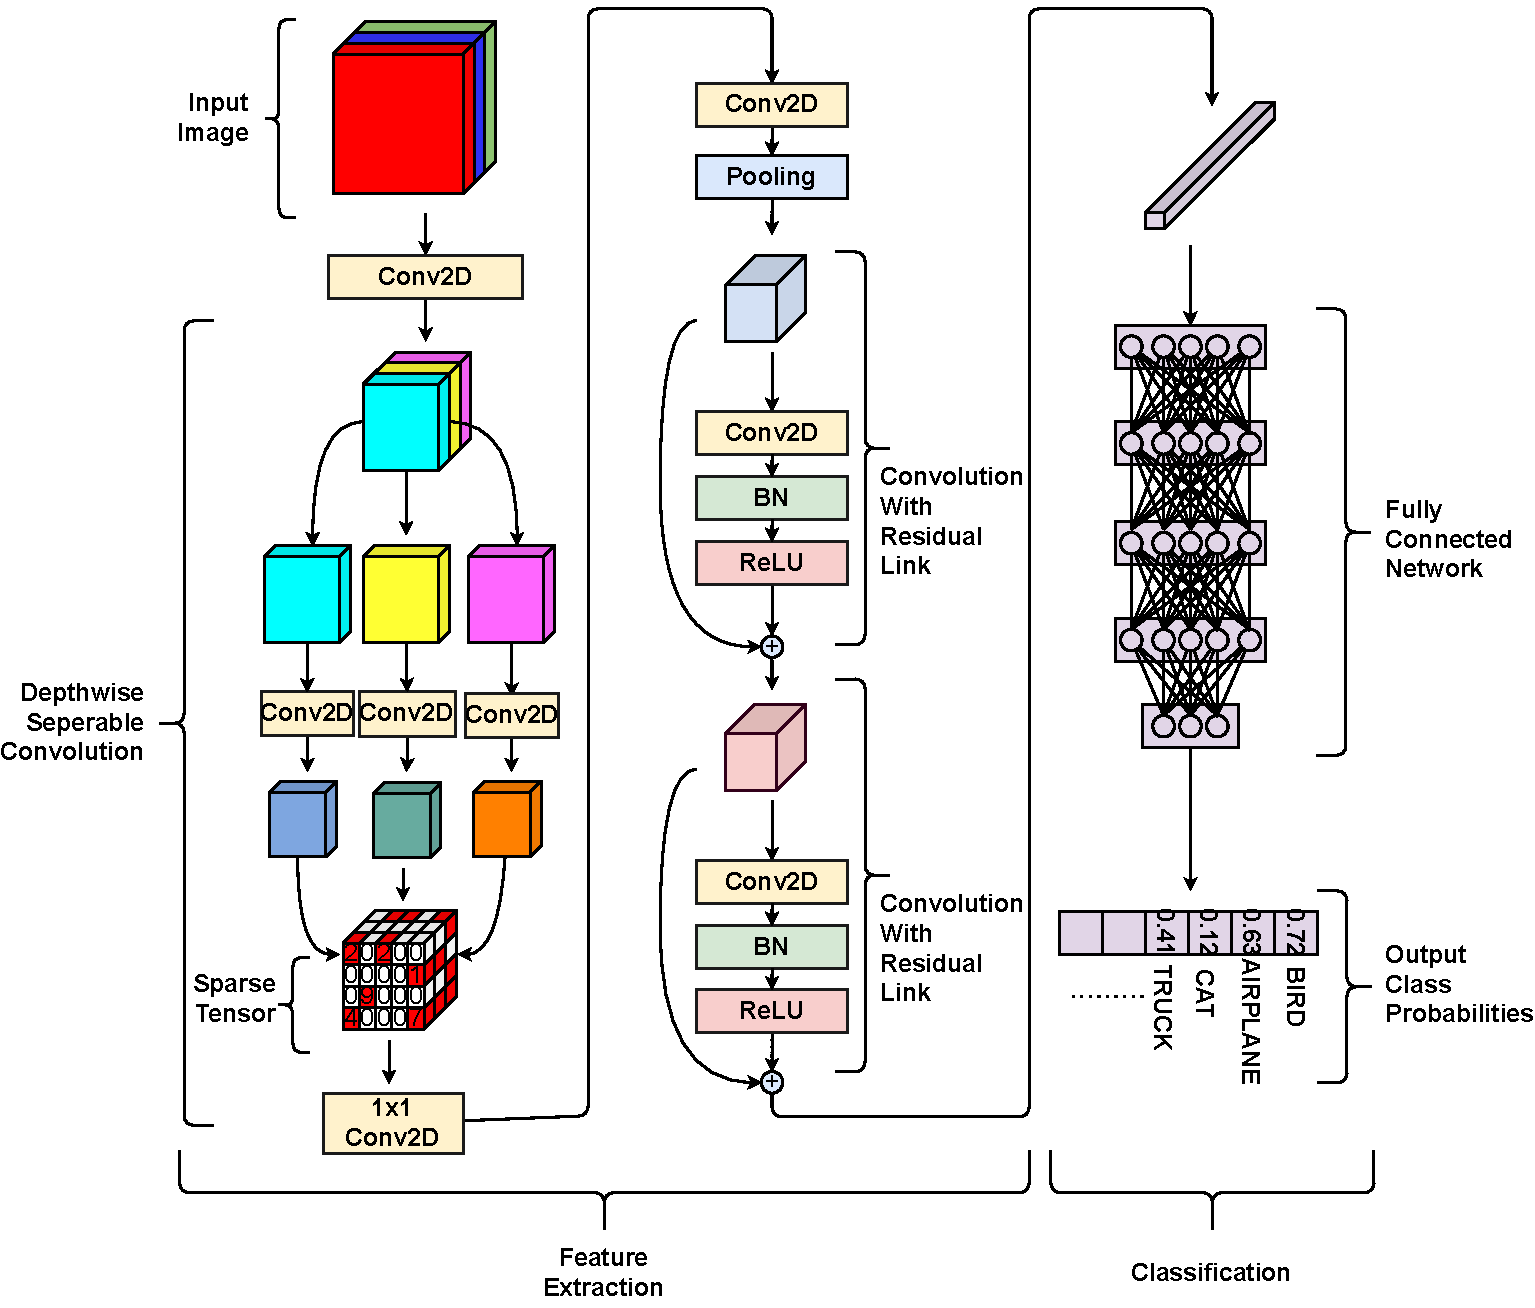
\includegraphics[scale=0.4]{fig/cnn.pdf}
    \caption{Example of the different layers in a convolution neural networks}
    \label{fig:cnn_network}
\end{figure}


Assuming the input feature map, output feature map and weight dimentionalities
of a layer are defined in \autoref{math:default_tensor_def}. A mathematical
representation of the convolution is given in \autoref{math:conv_equation_1fp}.
\autoref{math:conv_equation_1fp} represents a stencil based operation were a
sliding window called a kernel is moved accross an input feature and at each
position a multiply and accumulate operation is performed to compute an output
element of the output feature map. This stencil operation is repreated for each
kernel present in the layer. The number of kernels in a layer is called the
number of filters. This multiply and accumulate operate occurs accross the all
three dimensions of the IFmap tensor. In addition to the mathematical
description in \autoref{math:conv_equation_1fp} a visual representation of the
convolution operation is given in \autoref{fig:conv_explained}.

\begin{align}
    \begin{split}
        IFmap \in R^{C \times n\times n} \\
        OFmap \in  R^{F \times m\times m} \\
        Weight \in R^{F \times C\times K\times K} \\
    \end{split}
    \label{math:default_tensor_def}
\end{align}

\begin{align}
    OFmap[f][y][x] = \displaystyle\sum\limits_{c=0}^{C-1}\displaystyle\sum\limits_{k_x=0}^{K-1}\displaystyle\sum\limits_{k_y=0}^{K-1}Weight[f][c][k_y][k_x]*IFmap[c][y+ky][x+kx]
    \label{math:conv_equation_1fp}
\end{align}

\begin{figure}[ht]
    \centering
    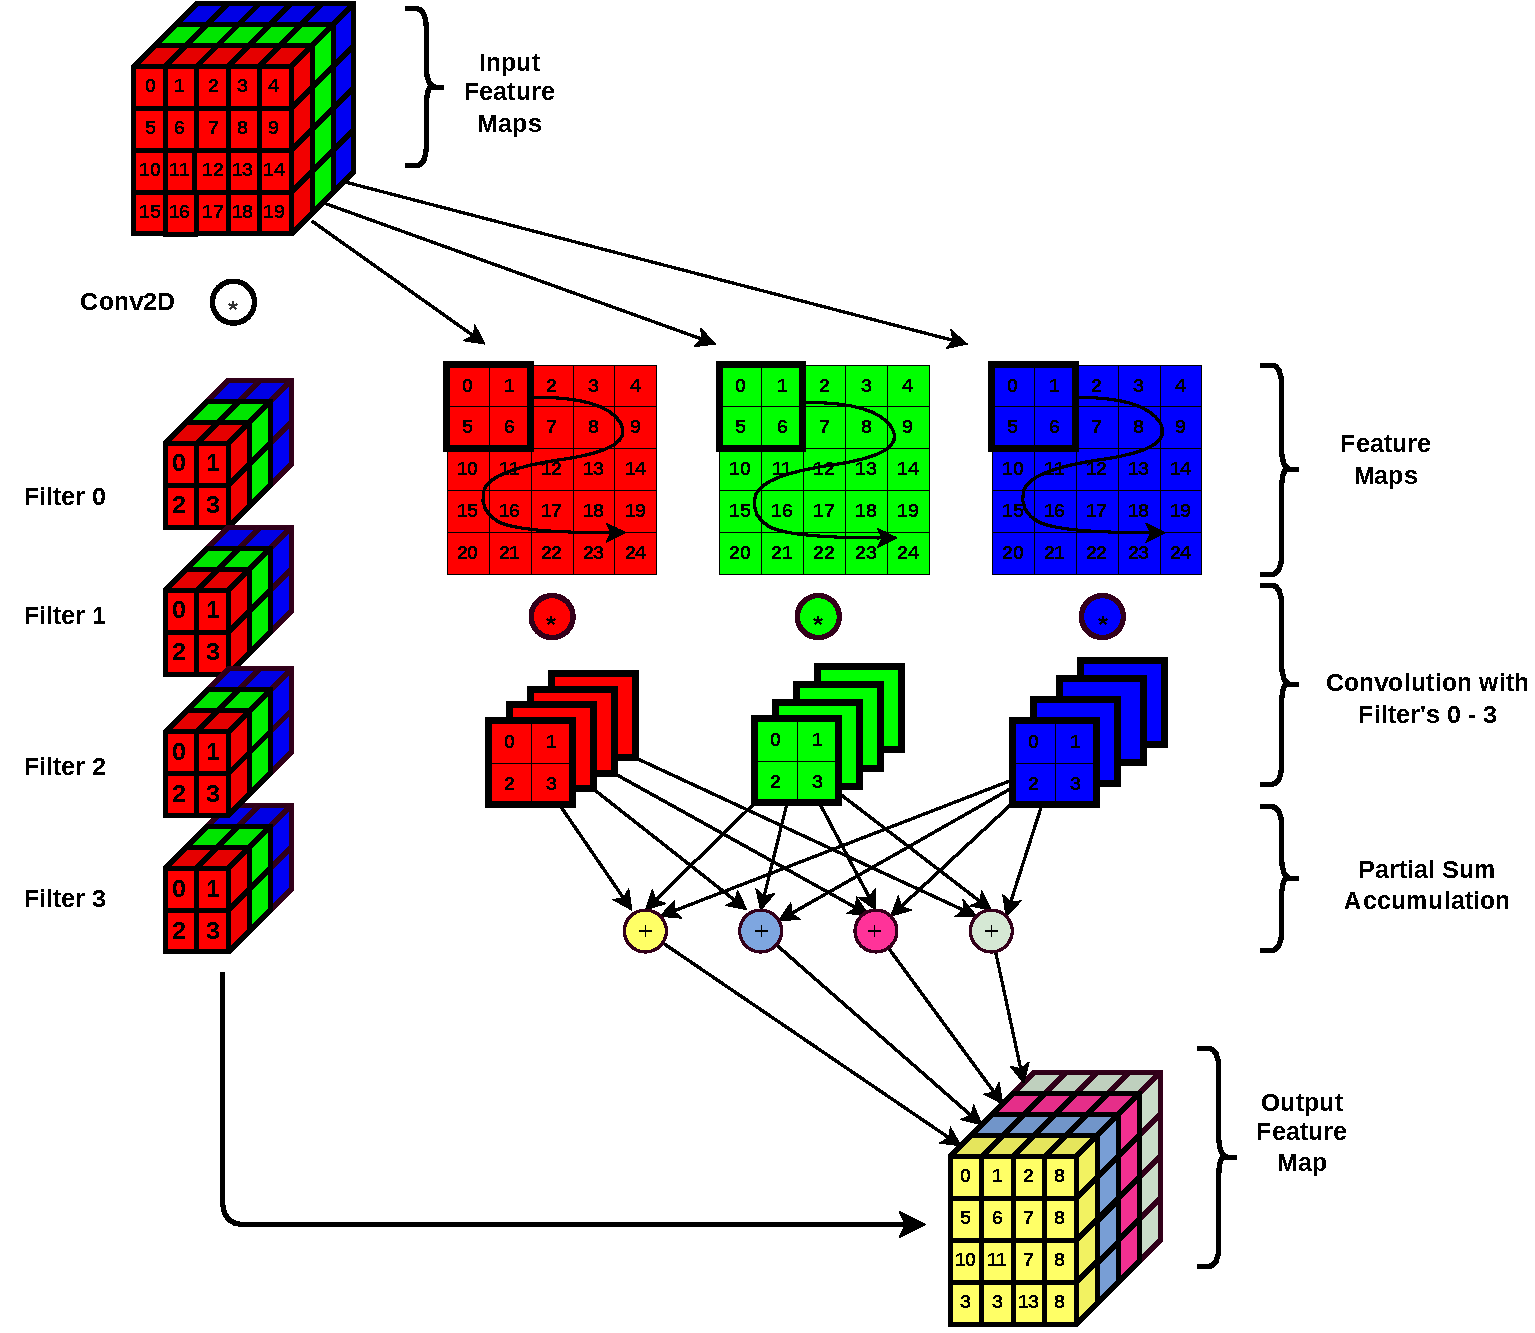
\includegraphics[scale=0.6]{fig/ConvExplained.pdf}
    \caption{Convolution Operation Illustrated}
    \label{fig:conv_explained}
\end{figure}

\section{Computing the convolution operation}
\label{chap:background:computing_conv}

To compute the convolution operation in software we can implement the expression
in \autoref{math:conv_equation_1fp} as a series of nested for loops as in
\autoref{lst:conv_loop}. This represents a direct approach to computing
convolution layers. However, this may not be an efficient way to compution
convolutions given the irregular access patterns inferred by the nested loops.
Irregular access patters may result in reduced performance due to inefficiencies
in a processors memory hierarchy. To mitigate this irregularity a transformation
can be applied to the inputs and ouputs of a convolution layer to convert the
overall operation into a general matrix multiplication which has a more regular
access pattern. In the literature
\cite{cafe_con_troll} there
are several different techniques used to perform this data transformation on the
inputs and outputs of a convolution layer.

\begin{minipage}{\linewidth}
    \begin{lstlisting}[language=C, caption=Convolution implemented as nested loops, label={lst:conv_loop}]
for(int f = 0; f < F; f++) // Filter loop
    for(int c = 0; c < C; c++) // Channel loop
        for(int y = 0; y < Y; y++) // Output feature map row
            for(int x = 0; x < X; x++)  // Output feature map col
                for(int ky = 0; ky < KY; ky++)  // Kernel row
                    for(int kx = 0; kx < KX; kx++)  // Kernel col
                        O[f][y][x] += I[c][y+ky][x+kx]*W[f][c][ky][kx];
    \end{lstlisting}
\end{minipage}

The first of the transformation techniques used in computing convolution
operations as general matrix multiplication discussed in \cite{cafe_con_troll}
is the Im2Col transformation or as \cite{cafe_con_troll} referes to it
"Expensive lowering/lifting". The lowering/ lifting nomenclature arises from
reduction of the IFmap and Weight tensor dimentionalities from 3D to 2D and vice
versa for the OFmap. The expensive descriptor arises from the substantial
increase in memory allocation required from lowering the IFmap input into two
dimensions as a result of data duplication. 

Expensive lowering and lifting "flattens" the IFmap by positioning a
hypothetical stencil where the real stencil would be positioned in the
convolution operation and collects all the IFmap elements present in that
stencil into one row of an IFmap matrix. This collection processes is repeated
for every real stencil position present in the original convolution operation.
Since stencil positions are usually very close to each other (depending on the
stride size of the layer) a substantial amount of IFmap elements are reused
between stencil positions. The act of lowering the contents of each stencil
position into one row results in the duplication of IFmap elemnents between
consecutive rows in the IFmap matrix.  
The weight kernels for each filter are flattened vertically into a weight
matrix. The OFmap matrix is then produced by matrix multiplcation between the
IFmap and weight matricies. To recover the OFmap tensor a "lifting" operation is
performed by reshaping the output OFmap matrix into a 3D tensor.  

\begin{figure}[ht]
    \centering
    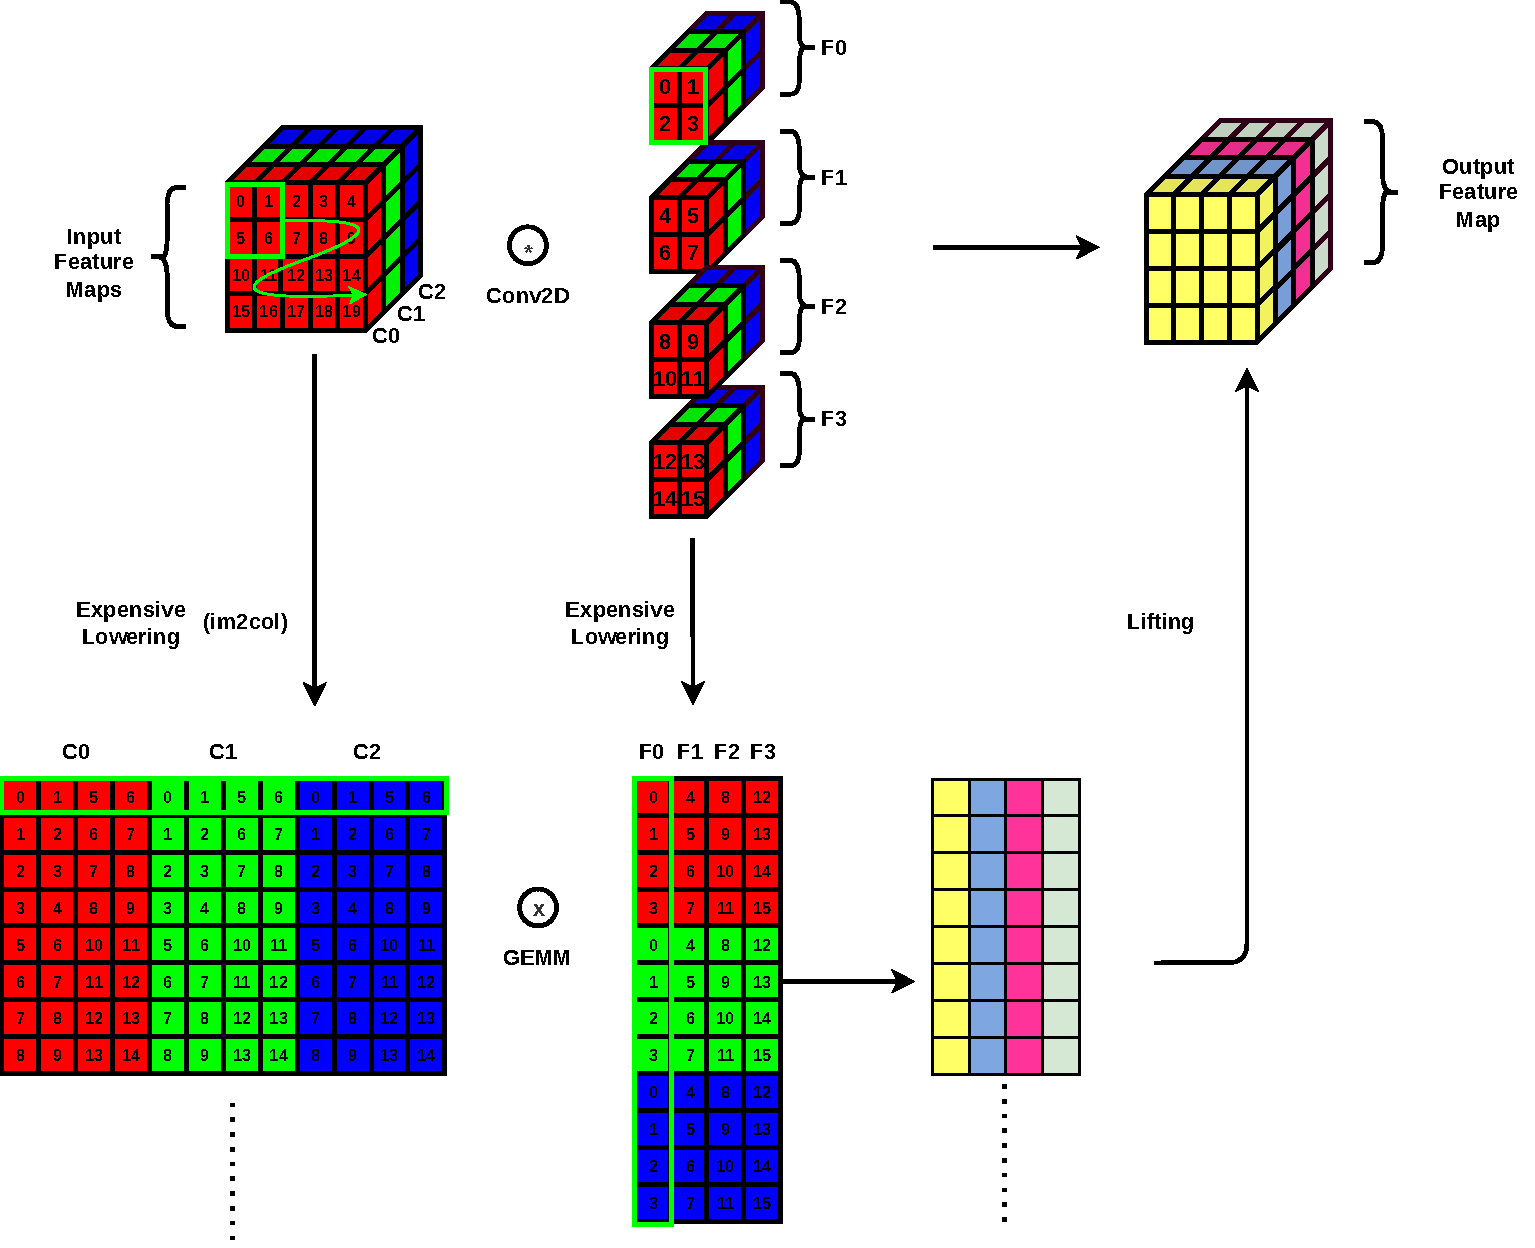
\includegraphics[scale=0.6]{fig/Im2Col.pdf}
    \caption{Im2Col (Expensive lowering/ lifting) Illustrated}
    \label{fig:im2col}
\end{figure}

An alternative approach to expensive lowering/ lifting is balanced lowering and
lifting. Balanaced lowering and lifting is a less visually intuitive data
transformation strategy. Therefore, analytical expressions adapted from
\cite{cafe_con_troll} are given in \eqref{math:balanced_lowering_ifmap} -
\eqref{math:balanced_lifting_ofmap} with the inclusion of lowering in
the presence of multiple filters to describe these data transformation
operations. In addition, to supplement the analytical expressions balanced
lowering presented \autoref{fig:balanced_lowering_lifting} is used to clarify
the available expressions further.  

In balanced lowering, we first lower the ifmap and weights using expression
\eqref{math:balanced_lowering_ifmap} and \eqref{math:balanced_lowering_weight}.
Then a matrix multiplication is performed in \eqref{math:balanced_lowering_gemm}
followed by a lifting operation. Unlike the lifting operation in the expensive
lowering/ lifting transformation, lifting in the balanced transformation
involves a series vector operation in addition to a reshape of the output OFmap
matrix. Balanced lowering has the advantage of reduced data duplication in the
IFmap and trades that off with increasing the number of FLOPs for lifting the
OFmap. 
 
\begin{align}
    \begin{gathered}
        IFmap \in R^{C\times n\times n} \xrightarrow[]{Balanced Lowering} \hat{IFmap} \in R^{nm\times KC} \\
        \hat{IFmap}[cn+r, :] = vec(IFmap[:, r, c:c+K]) \\
        \forall r,c \in [0, n-1], [0, m-1]
    \end{gathered}
    \label{math:balanced_lowering_ifmap}
\end{align}

\begin{align}
    \begin{gathered}
        Weight \in R^{F\times C\times K \times K} \xrightarrow[]{Balanced Lowering} \hat{Weight} \in R^{KC\times FK}\\
        \hat{Weight}[f*K:f*K+K, i] = vec(Weight[f, :, i, :]) \\
        \forall f,i \in [0, F-1], [0, K-1]
    \end{gathered}
    \label{math:balanced_lowering_weight}
\end{align}

\begin{align}
    \begin{gathered}
        \hat{OFmap} = \hat{IFmap}.\hat{Weight}
    \end{gathered}
    \label{math:balanced_lowering_gemm}
\end{align}

\begin{align}
    \begin{gathered}
        \hat{OFmap} \in R^{nm\times FK} \xrightarrow[]{Balanced Lifting} OFmap \in  R^{m\times m\times F}\\
        OFmap[f, r, c] = (\displaystyle\sum\limits_{j=0}^{K-1} \hat{OFmap}[cn+r+j, j+fK]) \\
        \forall f,r,c \in [0, F-1], [0, m-1], [0, m-1]
    \end{gathered}
    \label{math:balanced_lifting_ofmap}
\end{align}

\begin{figure}[!ht]
    \centering
    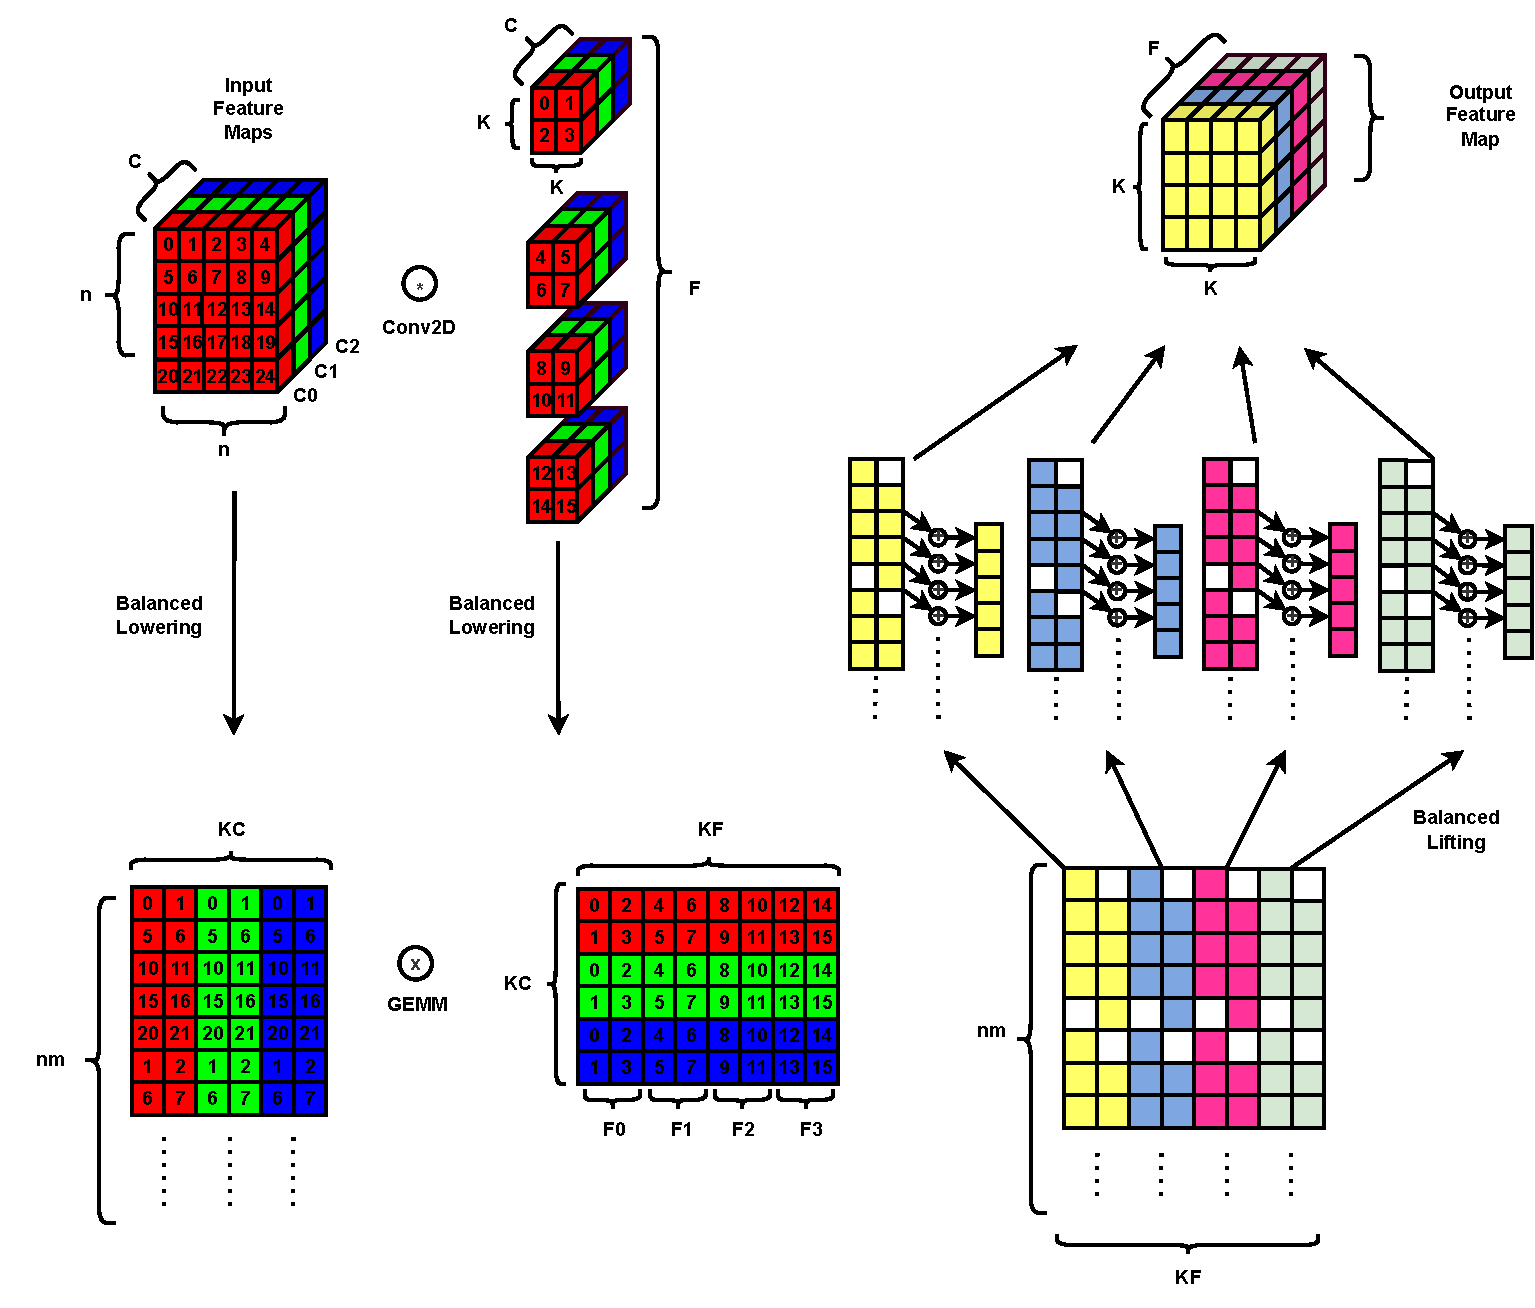
\includegraphics[scale=0.6]{fig/BalancedLoweringLifting.pdf}
    \caption{Balanced Lowering/Lifting Illustrated}
    \label{fig:balanced_lowering_lifting}
\end{figure}

The third (lowering/ expensive lifting) strategy further trades off the
the size of the lowered matricies by increasing the complexity of lifting.
However, this strategy diminished the gains from converting convolution layers
to general matrix multiplication and therefore are not elaborated on in this
thesis. \autoref{Table:lowering_lifting_breakdown} breakdown the
dimentionalities and complexities of the three strategies discussed in
\cite{cafe_con_troll} using the dimentions of the IFmap, OFmap, and Weight
tesnors defined in \autoref{math:default_tensor_def}.     


\begin{table}[]
    \begin{tabular}{ll|l|l|l|}
    \cline{3-5}
                                                                                                      &                     & \begin{tabular}[c]{@{}l@{}}Expensive \\ Lowering/ Lifting\end{tabular}   & \begin{tabular}[c]{@{}l@{}}Balanced \\ Lowering \\ and Lifting\end{tabular} & \begin{tabular}[c]{@{}l@{}}Lowering/ \\ Expensive Lifting\end{tabular} \\ \hline
\multicolumn{1}{|l|}{\multirow{2}{*}{Lowering}}                                                   & Lowered Data Size   & ($k^2$C, $m^2$)                                                              & (kC, mn)                                                                    & (C, $n^2$)                                              \\ \cline{2-5} 
    \multicolumn{1}{|l|}{}                                                                            & Lowered Kernel Size & (F, $k^2$C)                                                              & (Fk, kC)                                                                    & (F$k^2$, C)                                             \\ \hline
\multicolumn{1}{|l|}{\multirow{3}{*}{\begin{tabular}[c]{@{}l@{}}Matrix \\ Multiply\end{tabular}}} & Input Size          & (F, $k^2$C)x($k^2$C, $m^2$) & (Fk, kC)x(kC, mn)                              & (F$k^2$, C)x(C, $n^2$)                   \\ \cline{2-5} 
    \multicolumn{1}{|l|}{}                                                                            & \# FLOPS            & 2F$k^2$C$m^2$                                                            & 2F$k^2$Cmn                                                   & 2F$k^2$C$n^2$                            \\ \cline{2-5} 
    \multicolumn{1}{|l|}{}                                                                            & Output Size         & (F, $m^2$)                                                               & (Fk, mn)                                                                    & (F$k^2$, $n^2$)                          \\ \hline
    \multicolumn{1}{|l|}{\multirow{2}{*}{Lifting}}                                                    & \# FLOPS            & 0                                                                        & $m^2$kF                                                      & $m^2$$k^2$F                              \\ \cline{2-5} 
    \multicolumn{1}{|l|}{}                                                                            & \# Ram Read         & F$m^2$                                                                   & Fkmn                                                                        & F$k^2$$n^2$                              \\ \hline
    \end{tabular}
    \label{Table:lowering_lifting_breakdown}
    \caption{Breakdown of the dimensionalities and complexity (in FLOPs and Ram Reads) of the different available lowering and lifting strategies adapted from \cite{cafe_con_troll}}
\end{table}
    
\section{Implementing convolutions in hardware}
\subsection{The dataflow taxonomy}

In the dataflow design space, from \cite{dnn_df_overrated} 
dataflows can be represented using the direct convolution
nested loop structure combined with unroll pragmas. Listing \ref{lst:conv_loop} shows a generic
implementation of a single convolution layer as a loop structure under a weight
stationary dataflow configuration. What defines that dataflow is 1) loop unroll
targets 2) loop order 3) the unroll factors of the unrolled loops. Weight elements within a
kernel remain stationary throughout the computation of an output feature map
until a new tile of channels C\_T is loaded into the accelerator. Once the
weights within a particular channel and filter group are used to produce an
output feature map they are discarded and are only loaded again when computing
the same layer for a new input image. From listing \ref{lst:conv_loop} we
can see that from the loop unroll targets and loop unroll factors there are many
other possible dataflow configurations available to us outside of weight
stationary. Additionally, since accelerators are generally limited to two
spatial axis the loops of the convolution operation can be mapped to two spatial
axis. If we allow multiple convolution loops under some kernel unroll factor
KY\_T/KX\_T  to be unrolled and mapped to the same accelerator spatial axis we
can influence the effective unroll factors when performing different
convolutions of different kernel sizes other than KY\_T/KX\_T. The choice of
which loops are mapped to which spatial axis is an additional design dimension
alongside loop unrolling. To summarize, from the loop representation of
convolution accelerator dataflows we have three design space dimensions, 1. Loop
unroll targets 2. Loop unroll factors 3. Loop spatial mapping. 

\begin{minipage}{\linewidth}
    \begin{lstlisting}[language=C, caption=Convolution implemented as nested loops, label={lst:conv_loop}]
#pragma UNROLL F_T
for(int f = 0; f < F; f+=F_T) // Filter loop
#pragma UNROLL C_T
    for(int c = 0; c < C; c+=C_T) // Channel loop
#pragma UNROLL Y_T
        for(int y = 0; y < Y; y+=Y_T) // Output feature map row
#pragma UNROLL X_T
            for(int x = 0; x < X; x+=X_T)  // Output feature map col
#pragma UNROLL KY_T
                for(int ky = 0; ky < KY; ky+=KY_T)  // Kernel row
#pragma UNROLL KX_T
                    for(int kx = 0; kx < KX; kx+=KX_T)  // Kernel col
                        O[f][y][x] += I[c][y+ky][x+kx]*W[f][c][ky][kx];
    \end{lstlisting}
\end{minipage}

\subsection{The Hardware Implementation taxonomy}

\begin{figure}
    \centering
    \subfigure[]{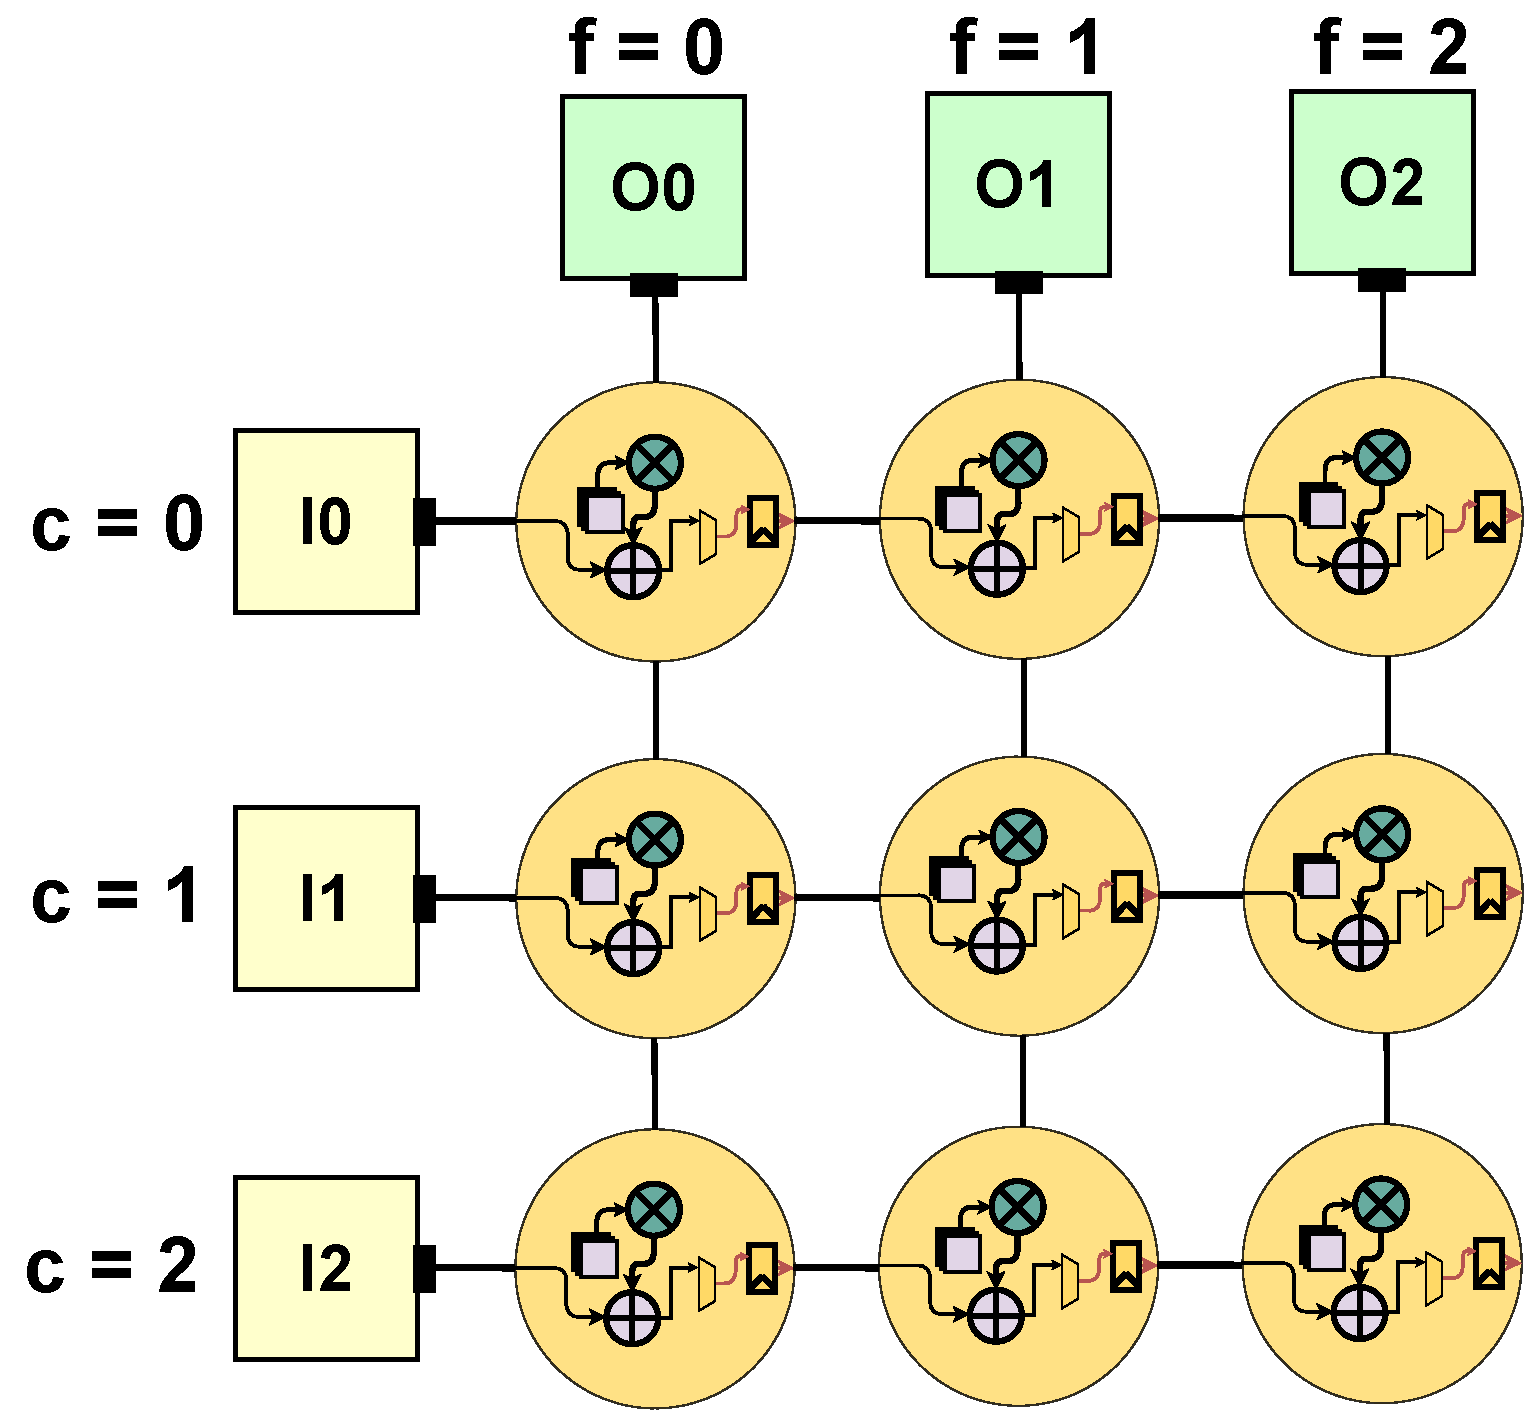
\includegraphics[width=0.32\textwidth]{fig/unroll_c_f.pdf}}
    \hspace{0.1cm} 
    \subfigure[]{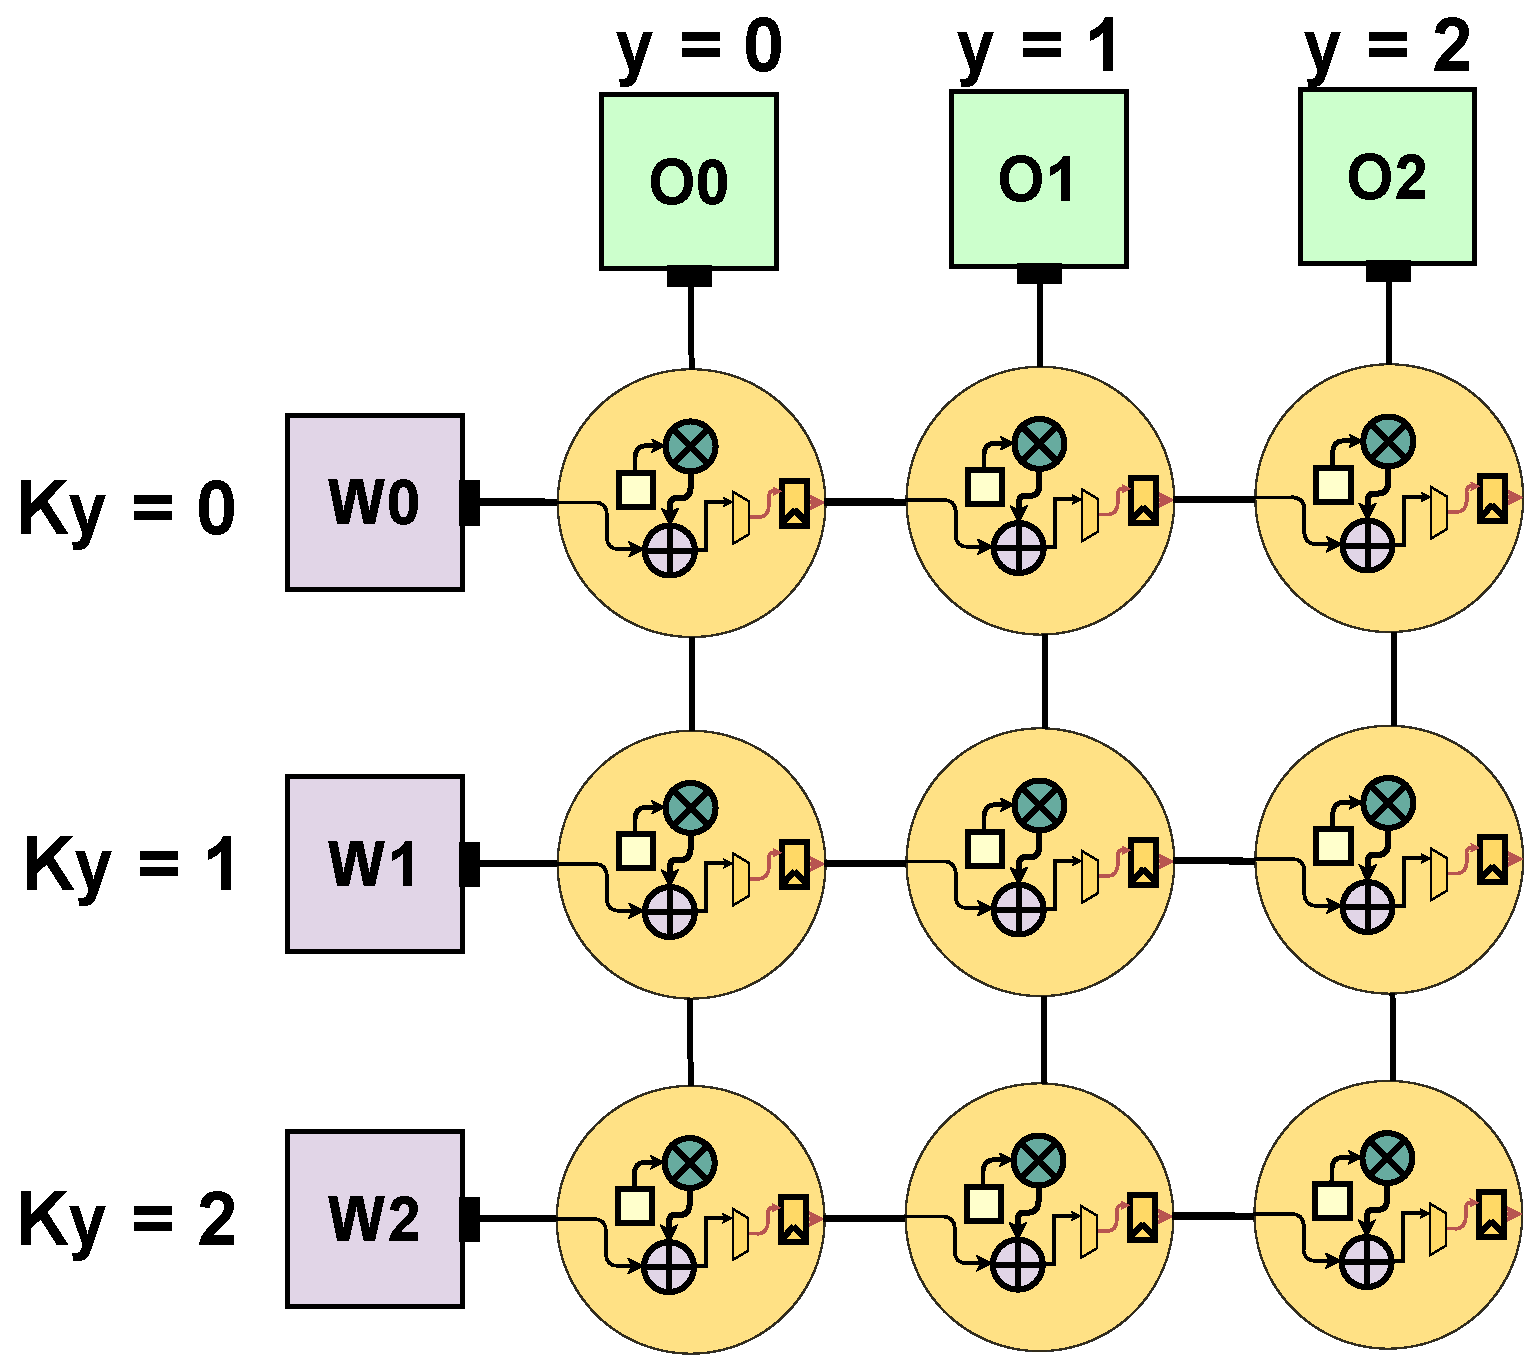
\includegraphics[width=0.32\textwidth]{fig/unroll_fy_y.pdf}}
    \hspace{0.1cm} 
    \subfigure[]{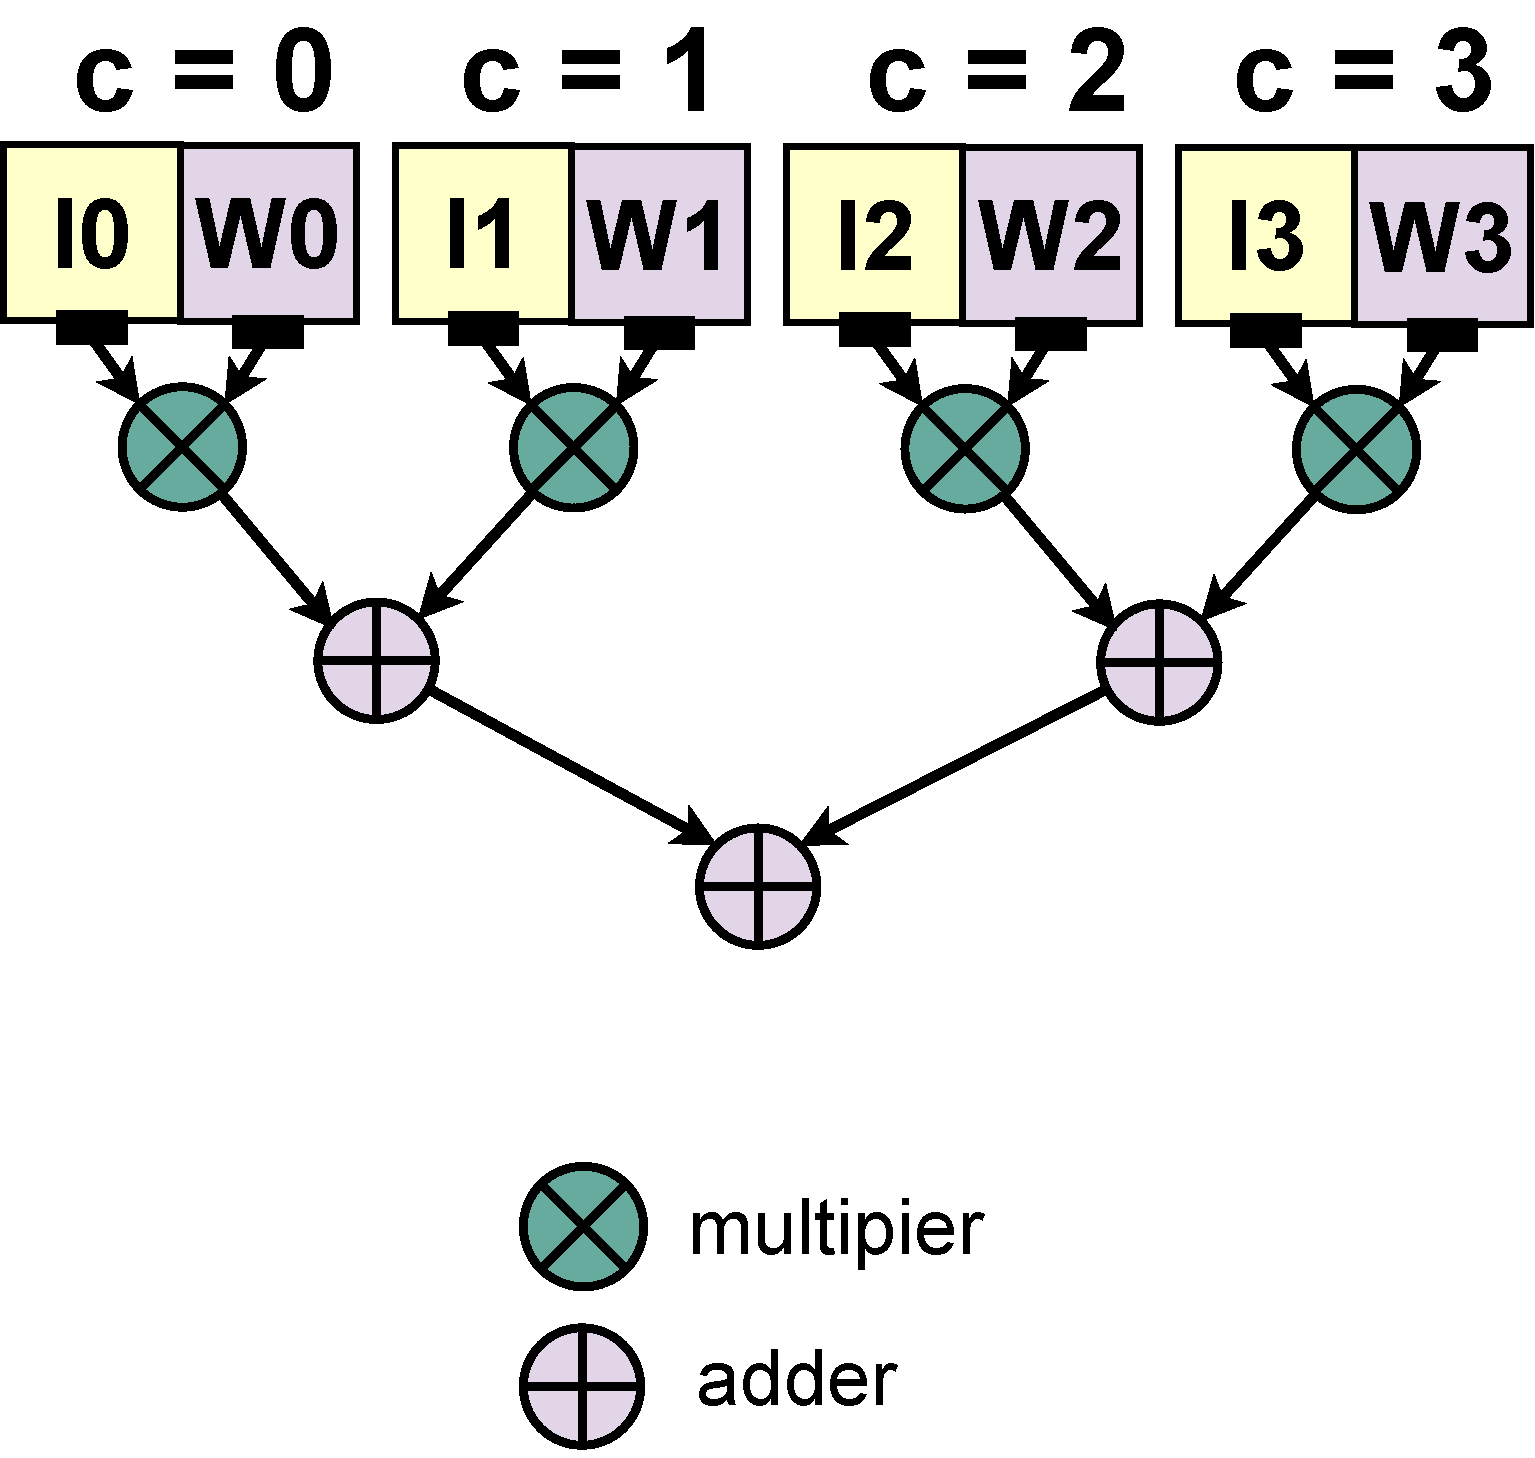
\includegraphics[width=0.32\textwidth]{fig/unroll_c.pdf}} 
    \hspace{0.1cm} 
    \subfigure[]{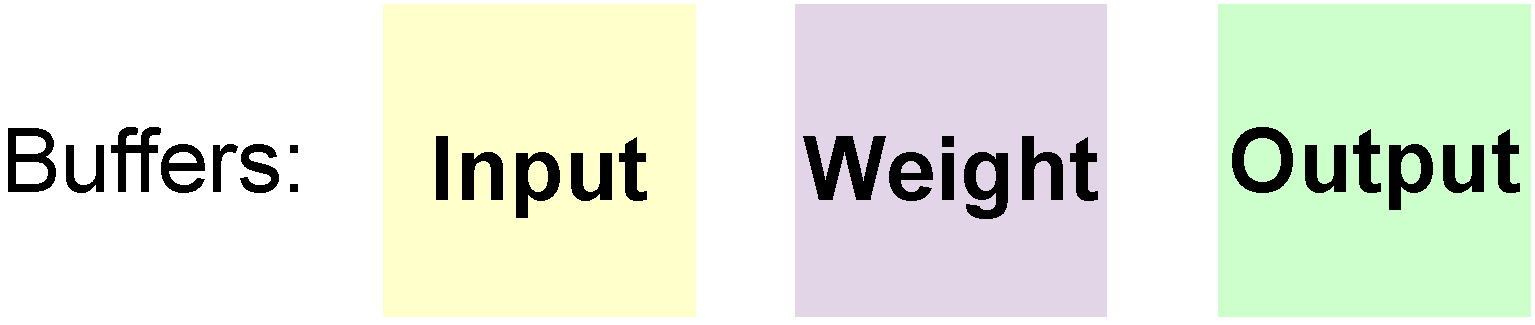
\includegraphics[width=0.3\textwidth]{fig/buffer_description.pdf}}
    \caption{Illustration of different dataflow implementations (adapted
    from\cite{dnn_df_overrated}) arising from (a) Unrolling F and C loops (b)
    unrolling Ky and Y loops (c) unrolling C loops}
    \label{fig:unroll_illustration}
\end{figure}

\begin{figure}[ht]
    \centering
    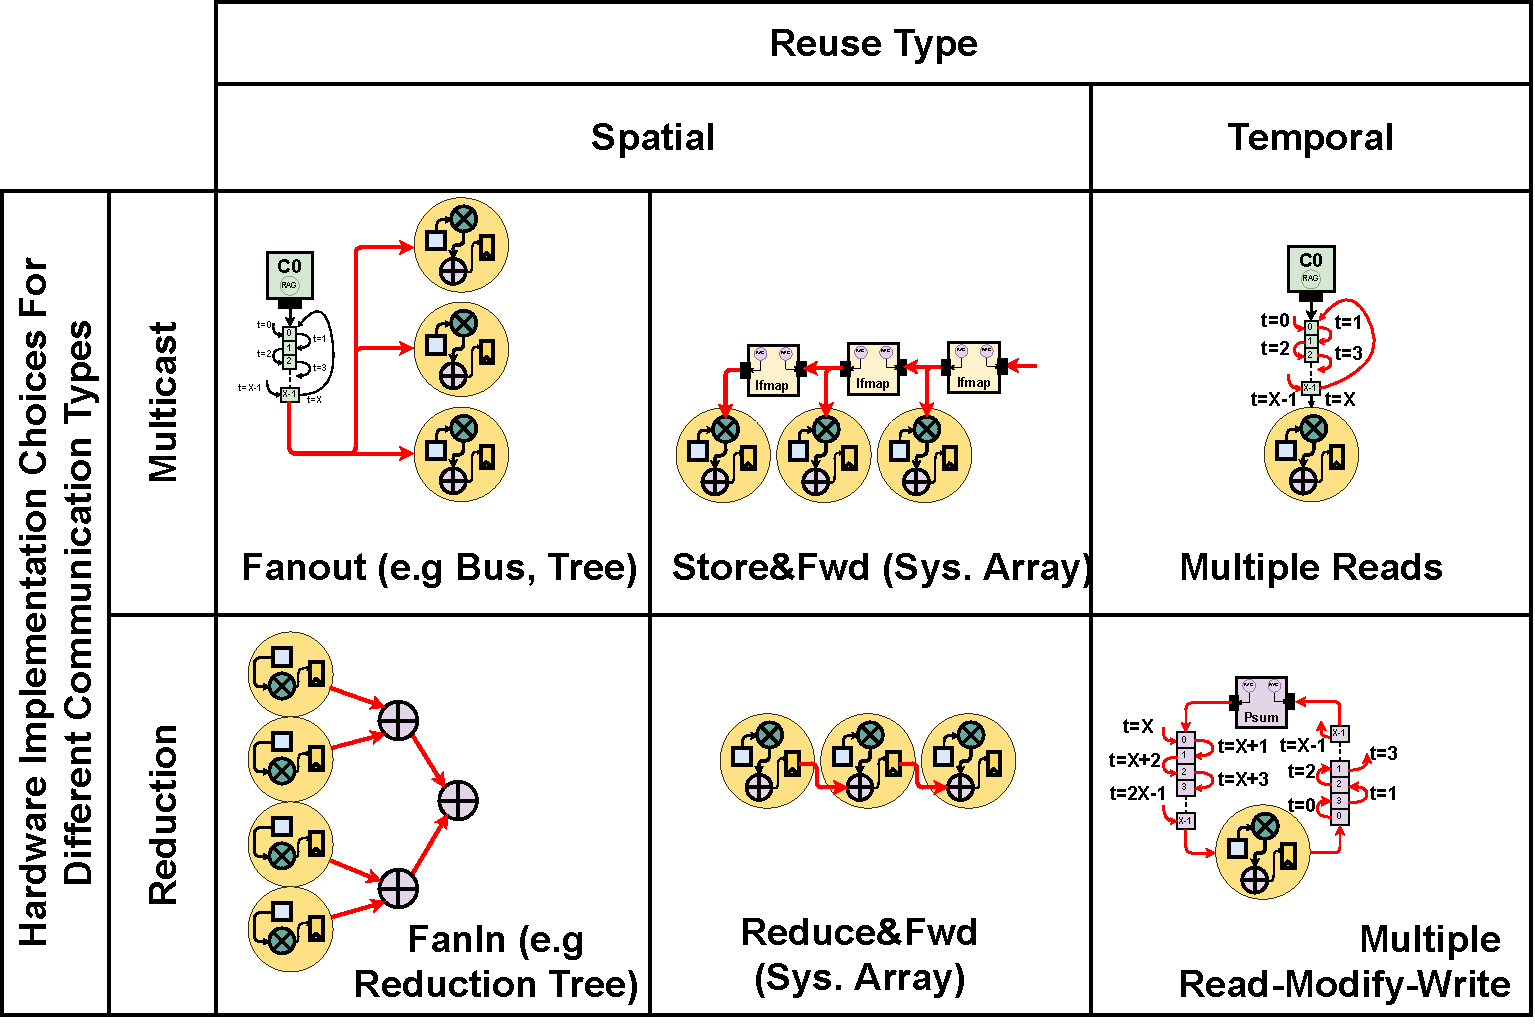
\includegraphics[scale=0.58]{fig/hw_taxonomy.pdf}
    \caption{Hardware Implementation Taxonomy adapted from \cite{maestro}}
    \label{fig:hw_taxonomy}
\end{figure}


Depending on the dataflow selected using the dataflow taxonomy (1) loop ordering
(2) unroll targets (2) loop unroll factors. The implementation options are
derived based on the type of reuse present in the dataflow. Following the
hardware implementation taxonomy presented in in \cite{maestro}, we can classify
the available hardware implementation options based on the the type of reuse is
spatial where a data element is read and used in the same cycle or temporal
where a data element is read in one cycle and reused after several cycles.
Depending on the nature of the reuse, if it is read or read modify write, there
are several options for supporting the communication inferred from that reuse
type. To deduce the type of reuse and overall communicaiton behavior for each
data element in any dataflow we can use the polyhedral model to detect temporal
reuse. Spatial reuse detection can be inferred directly from the loops. The
application of the polyhedral to infer temporal reuse behavior as well as the
inference of spatial reuse directly from the convolution loops is discussed in
\autoref{chap:dda}.

Figures in \autoref{fig:unroll_illustration} show different reduction/ multicast
schemes based on reuse behavior of data elements (IFmap, OFmap, Weights)
apparent in the dataflow. The space of available schemes is not limited to those
presented in \autoref{fig:unroll_illustration} though. In \cite{maestro} a
hardware taxonomy illustrated in figure \autoref{fig:hw_taxonomy}.

\section{Related work}
\label{chap:related_work}

To contrast this work with other works in the literature a brief discussion of
competing accelerator designs is presented in this section. Note that the
related works discussion is limited to competing accelerator designs meant for
ASIC based implementations. Convolution accelerator generators targeting FPGAs
are not discussed here.

\subsection{Eyeriss V1 and V2}
\label{chap:related_work:eyeriss}

Eyeriss \cite{isscc_2016_chen_eyeriss} is an accelerator for state-of-the-art
deep convolutional neural networks (CNNs). It attempts to optimize for the
energy efficiency of the entire system by minimizing data movement between the
accelerator and DRAM thus reducing data movement energy. Eyeriss achieves these
goals by using a the row stationary (RS) dataflow on a spatial architecture with
168 processing elements. 

EyerissV2 \cite{eyerissv2} improve on EyerissV1 by proposing an architecture
optimized for sparse and compact DNNs. To account for the substantial variation
between different CNN layer it introduces a highly flexible on-chip network,
called hierarchical mesh, that can adapt to the different amounts of data reuse
and bandwidth requirements of different data types. THe goal of the mesh is to
improve the utilization of the computation resources.

EyerissV1 and EyerissV2 do not optimize for linear layers. Linear layers may not
represent a substantial portion of a CNN network runtime, however, some models
use linear layers exclusively. These models are underepresented in vision based
tasks however, they are present in NLP based tasks. An examples of these
models includes the Transformer model \cite{transformer_model}. This limits how general the
Eyeriss architecture is when used for models outside of the vision domain. This
work aims to build an accelerator that accounts for the importance of linear
layers in those models. 

\subsubsection{Tensor processing unit}
\label{chap:related_work:tpu  }

At the heart of a TPU is a 65,536 8-bit MAC matrix multiply unit that offers a
peak throughput of 92 TeraOps/second (TOPS) and a large (28 MiB)
software-managed on-chip memory \cite{tpu}. The TPU emphasizes efficiency in
computing matrix multiplcation above all other operations. With the
afformentioned transformations used to convert convolution layers to general
matrix multiplication the TPU is able to accelerate a wide variety of
computation workloads given the generality of the operation it's hardware
accelerates. This generality comes at the cost of efficiency in computing
convolution layers given the overheads of the transformations discussed in the
prior sections. This works aims to mitigate this inefficiency while maintaing
support for a wide variety of computation workloads. 


\subsection{Maeri}
\label{chap:related_work:maeri}

Since most DNN accelerators support only fixed dataflow patterns internally
mapping arbitrary layer dataflows to these fabric efficiently is challenging.
Mapping inefficiencies can lead to underutilization of the available compute
resources. DNN accelerators need to be configurable internally to support the
various dataflow patterns that could be mapped over them. To address this
\cite{maeri} introduces MAERI, a DNN accelerator built with a set of modular and
configurable building blocks backed by a flexible on-chip network capable of
supporting a myriad of DNN partitions and mappings. 

MAERI aims to support a wide variety of DNN layers and mappings by moving the
complexity of data orchestration to runtime configuration of a flexible on-chip
NOC. The drawback of this approach is the complexity of the NOC as well as the
area it occupies on-chip. This work aims to combine the runtime flexibility of
data orchestration on-chip through the use of a novel data orchestration
primitive called self addressable memory (SAMs) discussed in
\autoref{chap:data_orchestration} with the small area footprint of a fixed
on-chip fabric optimized through a novel optimizer presented in
\autoref{chap:arch_dimensioning}. 


% \section{Analysis of data reuse with the polyhedral model}

% \cite{meeus} used polyehdral model to analyse reuse within stencil based applications described
% as nested loops. One important element in their approach is their program written in iscc that
% can determine temporal reuse of data elements

% There's the polyhedral extraction tool out there but unfortunately there's no
% way to encode parallelism or loop unrolling in it without relying on compiler
% pragmas. 

% below is an example of this reuse applied to the gemm loops
